\label{timeline}
\begin{figure*}[t]
	\centering
	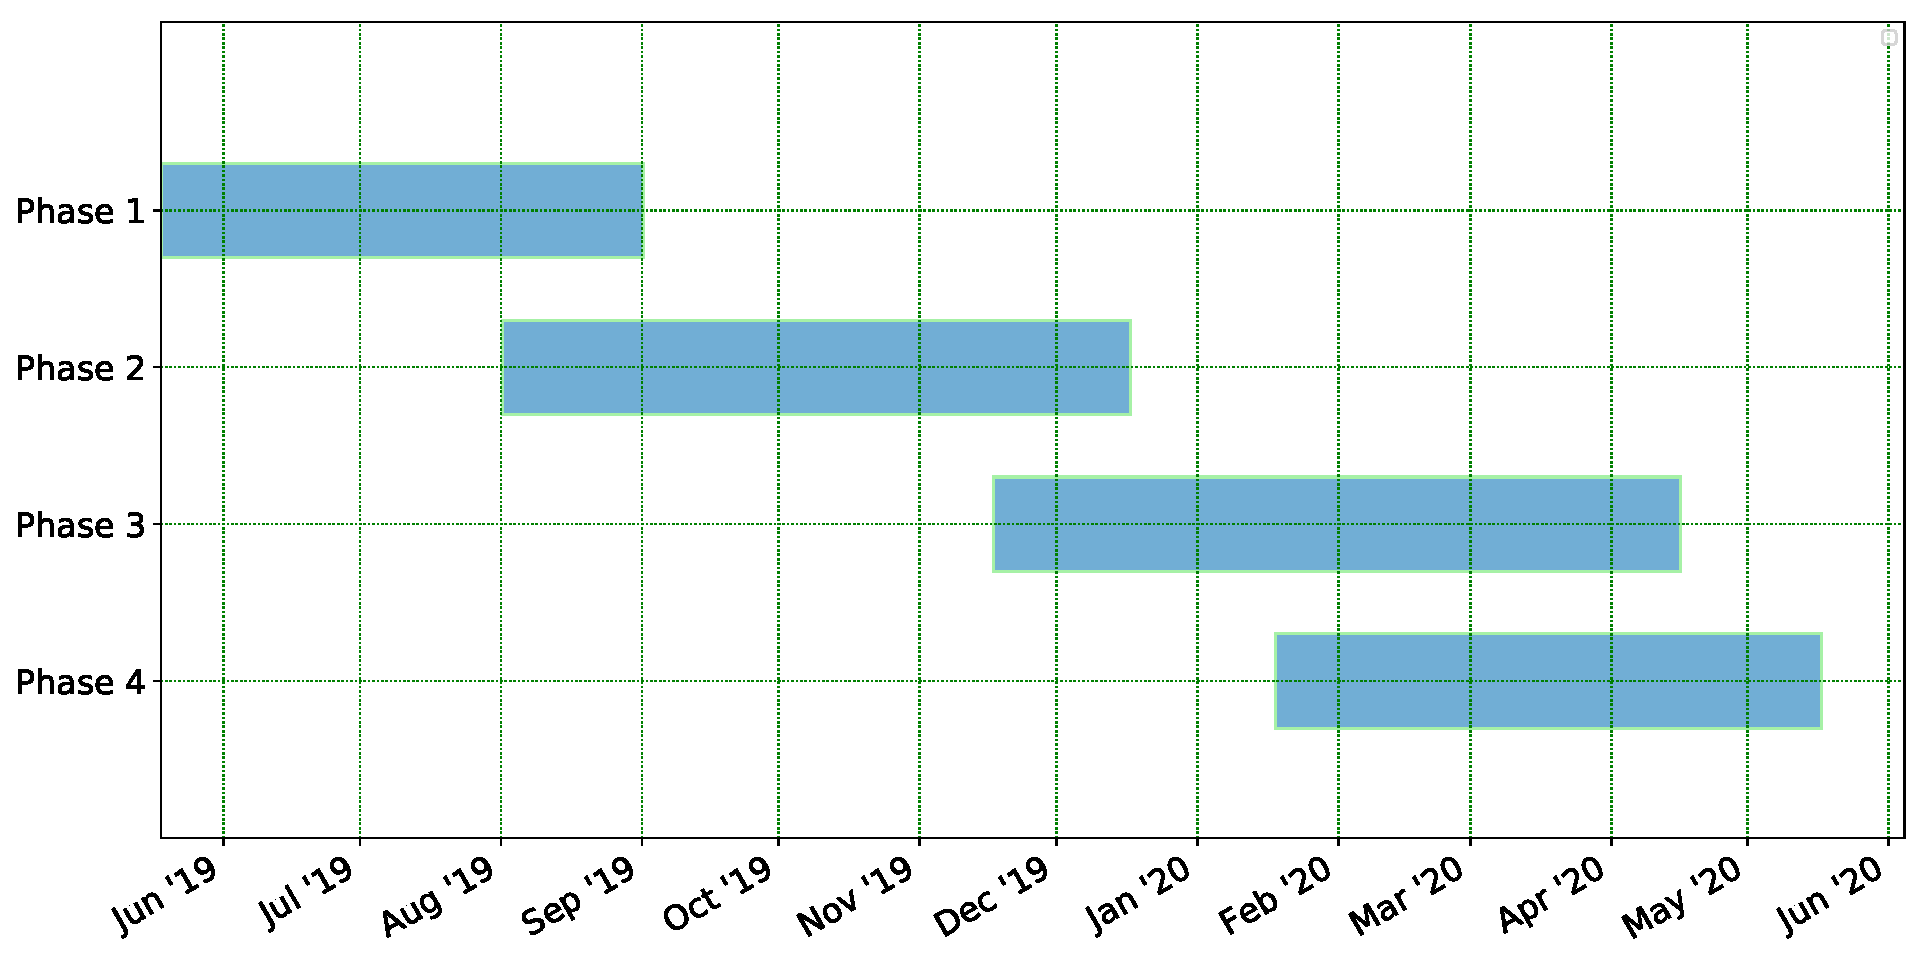
\includegraphics[width=.95\textwidth]{figures/phd_plan.pdf}
	\caption{Planned timeline of proposed research}\label{fig:work_plan}
\end{figure*}

\subsubsection{Phase 1: Design and implementation self-configuring property}

Month 1 would include design discussions for a prototype of the execution system. 
Result of these discussions will be the requirements of the middleware and its 
API. Design will be finalized and a prototypical implementation will be completed 
by Month 4. Capability to self-configure in terms of resources based on the desired 
workflow will mark the success of Phase 1.

\subsubsection{Phase 2: Implementation self-monitoring, self-regulating properties
and Continuous Integrated Testing}
Phase 2 includes defining the requirements for self-monitoring, and self-regulating 
properties and implement them in the middleware. End of phase 2 will include the 
\textit(self-*) properties as well as a Continuous integrated testing protocol to 
always verify the functionality of the middleware. Phase 2 spans from months 3 up 
to 6

\subsubsection{Phase 3: Integration with scientific workflows}
Phase 3 of the plan includes the integration of the proposed autonomic system with 
RADICAL-EnTK~\cite{balasubramanian2018harnessing} and start utilize the system for 
scientifc workflows in Satelite Imagery analysis and Molecular Dynamics simulation 
workflows. This phase spans between months 6 and 9.

\subsubsection{Phase 4: Investigation for an empirical model}

Experiments with synthetic and real applications with the prototype as well as 
scientific workflows will be used to investigate and derive empirical models. 
These models may be used to further generalize the behavior of the autonomic 
middleware based on application requirements. Phase 4 will overlap with Phase 2 
and 3 to utilize experiments done during those phases.

% ---------------------------------------------------------------------------
% Why
\subsection{Significance and impact of work}
Several scientific applications are required to be executed several times with 
different input data or initial conditions. The required concurrency to minimize 
the execution time of each run is not necessarily constant and may change based 
on the initial conditions. The autonomic management system suggested in this 
proposal will be the first to make resource configuration decisions for the users. 
This will lead to less time invested by users to make execution decisions about 
their workflows. These decisions will lead to better resource utilization and, 
as a result, better domain science. The empirical models derived by this work can 
be used to derive formal mathematical models.

% ---------------------------------------------------------------------------
% Challenges
\subsection{Challenges/Risks}

We estimate the proposed work, divided into four major phases, to take 12 months 
and we allocate 3 months to account for unforeseen circumstances. We would like 
to keep the committee aware of the following challenges that we see:

\begin{itemize}
	\item Design and Implementation (phases 1 \& 2) is iterative and special attention 
	needs to be given to the number of iterations against specific objectives, 
	given the timeline.
  \item All experiments performed on HPC systems are subject to variable queue 
	times and may limit the number of experiments performed in phase 2 and 4.
	\item Although the middleware will be well tested (80--90\% of the code base 
	will be covered by unit tests) and less susceptible to major changes, RADICAL-Pilot 
	is known to be less stable and is susceptible to changes as it serves multiple 
	projects. Stability of RADICAL-Pilot is considered in the estimates, but needs 
	to be made aware to the committee.
	\item Lastly, the HPC systems themselves may often become inaccessible due to 
	unplanned outages.
\end{itemize}